% !TEX root =../prj4projektrapport.tex

\section{Belastning}

Til simulering af forbrugere i systemet er ohmske belastninger benyttet. Modstandsværdierne for disse er valgt i intervallet 16$\Omega$ til 100$\Omega$, da disse vil give tilstrækkeligt spændingsfald, $\pm$10$\%$ af 4V, til at medføre trinskift\footnote{Projektdokumentation, 8.2.1, Beregning af Belastning}. 

\subsection{Design og implementering}

I systemet er de førnævnte belastninger placeret i parallel, og til hver belastning hører en kontakt, der giver mulighed for nemt at til- og frakoble forskellige belastninger. I serie med hver belastning sidder en 1 $\Omega$ modstand for at kunne tilkoble en Måleenhed til overvågning. Det færdige print med belastninger ses på figur \ref{fig:Belastning}. Nederst til venstre på printet ses pin, der kobles til distributionslinjen. Øverst til venstre ses bananstik, der kobles til 0V på trintransformeren. 

\begin{figure}[H]
	\centering
	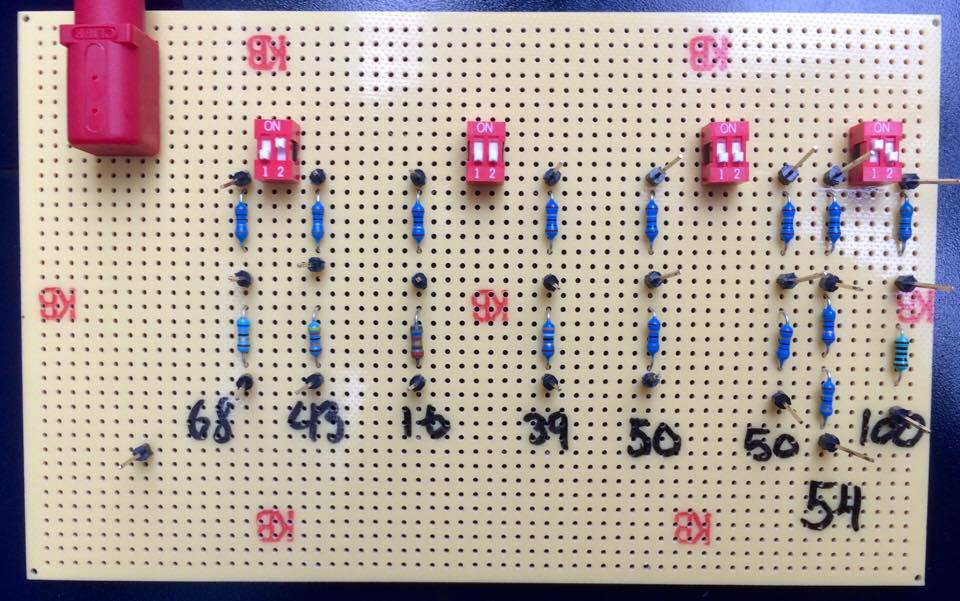
\includegraphics[width=0.6\textwidth]{figure/Belastningskreds}
	\caption{Færdigt print med belastninger}
	\label{fig:Belastning}
\end{figure}